%%%%%%%%%%%%%%%%%%%%%%%%%%%%%%%%%%%%%%%%%
% Short Sectioned Assignment
% LaTeX Template
% Version 1.0 (5/5/12)
%
% This template has been downloaded from:
% http://www.LaTeXTemplates.com
%
% Original author:
% Frits Wenneker (http://www.howtotex.com)
%
% License:
% CC BY-NC-SA 3.0 (http://creativecommons.org/licenses/by-nc-sa/3.0/)
%
%%%%%%%%%%%%%%%%%%%%%%%%%%%%%%%%%%%%%%%%%

%----------------------------------------------------------------------------------------
%	PACKAGES AND OTHER DOCUMENT CONFIGURATIONS
%----------------------------------------------------------------------------------------

\documentclass[paper=a4, fontsize=11pt]{article} % A4 paper and 11pt font size

    \usepackage[margin=2.5cm]{geometry}
    \usepackage[T1]{fontenc} % Use 8-bit encoding that has 256 glyphs
    \usepackage{fourier} % Use the Adobe Utopia font for the document - comment this line to return to the LaTeX default
    \usepackage[english]{babel} % English language/hyphenation
    \usepackage{amsmath,amsfonts,amsthm} % Math packages
    \usepackage{graphicx}
    \usepackage{lipsum} % Used for inserting dummy 'Lorem ipsum' text into the template
    \usepackage{listings}
    \usepackage{sectsty} % Allows customizing section commands
    \usepackage{float}
    \usepackage{physics}
    \allsectionsfont{\centering \normalfont\scshape} % Make all sections centered, the default font and small caps
    
    \usepackage{fancyhdr} % Custom headers and footers
    \pagestyle{fancyplain} % Makes all pages in the document conform to the custom headers and footers
    \fancyhead{} % No page header - if you want one, create it in the same way as the footers below
    \fancyfoot[L]{} % Empty left footer
    \fancyfoot[C]{} % Empty center footer
    \fancyfoot[R]{\thepage} % Page numbering for right footer
    \renewcommand{\headrulewidth}{0pt} % Remove header underlines
    \renewcommand{\footrulewidth}{0pt} % Remove footer underlines
    \setlength{\headheight}{13.6pt} % Customize the height of the header
    
    \numberwithin{equation}{section} % Number equations within sections (i.e. 1.1, 1.2, 2.1, 2.2 instead of 1, 2, 3, 4)
    \numberwithin{figure}{section} % Number figures within sections (i.e. 1.1, 1.2, 2.1, 2.2 instead of 1, 2, 3, 4)
    \numberwithin{table}{section} % Number tables within sections (i.e. 1.1, 1.2, 2.1, 2.2 instead of 1, 2, 3, 4)
    
    \setlength\parindent{0pt} % Removes all indentation from paragraphs - comment this line for an assignment with lots of text
    
    %----------------------------------------------------------------------------------------
    %	TITLE SECTION
    %----------------------------------------------------------------------------------------
    
    \newcommand{\horrule}[1]{\rule{\linewidth}{#1}} % Create horizontal rule command with 1 argument of height
    
    \title{	
    \normalfont \normalsize 
    \textsc{University of Oslo, Department of Mathematics} \\ [25pt] % Your university, school and/or department name(s)
    \horrule{0.5pt} \\[0.4cm] % Thin top horizontal rule
    \huge Mandatory assignment 1: MEK4470 \\ % The assignment title
    \horrule{0.5pt} \\[0.5cm] % Thin bottom horizontal rule
    }
    
    \author{Trym Erik Nielsen} % Your name
    
    \date{\normalsize\today} % Today's date or a custom date
    
    \begin{document}
    \lstset{language=Python}
    
    \maketitle % Print the title
    
    %----------------------------------------------------------------------------------------
    %	PROBLEM 1
    %----------------------------------------------------------------------------------------
    
    \section*{Excercise 1}
    TVD schemes stand for Total Variation diminishing schemes. TVD attempts to reduce "wiggles" in the numerical solution, by limiting numerical diffusion in the solution. In this exercise, we have attempted to introduce a Van-Leer flux limiter TVD scheme using Central Differencing for the convection, in the one dimensional convection diffusion problem. Below follows the computed results for the transport of $\phi$ (top graph), and the $L_2$ computed norm (bottom graph)

    \begin{figure}[h!]
        \centering
        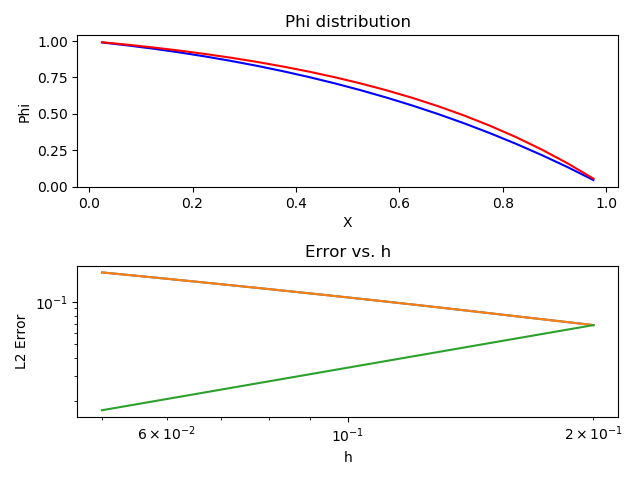
\includegraphics[width=0.6\linewidth]{Figures/ConvectionDiffusion}
        \caption{Top: Steady state solution $\phi$, bottom: $L_2$ error}
        \label{fig:ConvDiff}
    \end{figure}        

    We can see from the top graph of figure \ref{fig:ConvDiff} that we have a reasonable fit with the analytical solution (red) and the computer solution (in blue). However, we do not see convergence in $L_2$. The log-log graph of the $L_2$ error versus the cell size shows in an inverse relationship. For convergence of the solution in $L_2$ we expect $L_2$ to linearly decrease (on a log-log plot) against smaller cell size. The suspected reason for this is due to the authors difficulty in modelling the ratio of the upstream gradient with the downstream gradient, as well as accounting for all fluxes accross the control volume faces. Refer to appendix for the python code used in this example.  

    
    %----------------------------------------------------------------------------------------
    %	PROBLEM 2 - part 1
    %----------------------------------------------------------------------------------------
    \clearpage
    \section*{Excercise 2}
    \subsection*{part 1}

    \lstset { %
    language=C++,
    basicstyle=\footnotesize,% basic font setting
    }

    \begin{lstlisting}[language=C++, captionpos = b, caption=Source code for pisoFoam]    
      #include "fvCFD.H"
      #include "singlePhaseTransportModel.H"
      #include "turbulentTransportModel.H"
      #include "pisoControl.H"
      #include "fvOptions.H"
      
      // * * * * * * * * * * * * * * * * * * * * * * * * * * * * * * * * * * * * * //
      
      int main(int argc, char *argv[])
      {
          #include "postProcess.H"
      
          #include "setRootCase.H"
          #include "createTime.H"
          #include "createMesh.H"
          #include "createControl.H"
          #include "createFields.H"
          #include "createFvOptions.H"
          #include "initContinuityErrs.H"
      
          turbulence->validate();
      
          // * * * * * * * * * * * * * * * * * * * * * * * * * * * * * * * * * * * //
      
          Info<< "\nStarting time loop\n" << endl;
      
          while (runTime.loop())
          {
              Info<< "Time = " << runTime.timeName() << nl << endl;
      
              #include "CourantNo.H"
      
              // Pressure-velocity PISO corrector
              {
                  #include "UEqn.H"
      
                  // --- PISO loop
                  while (piso.correct())
                  {
                      #include "pEqn.H"
                  }
              }
      
              laminarTransport.correct();
              turbulence->correct();
      
              runTime.write();
      
              Info<< "ExecutionTime = " << runTime.elapsedCpuTime() << " s"
                  << "  ClockTime = " << runTime.elapsedClockTime() << " s"
                  << nl << endl;
          }
      
          Info<< "End\n" << endl;
      
          return 0;
      }

      // ************************************************************************* //
    \end{lstlisting}
    \clearpage
    
    The Piso algorithm follows the following structure

    \begin{itemize}
        \item Solve the discretized momentum equation
        \item Solve pressure correction equation
        \item Correction of pressure and velocities
        \item solve for second pressure correction
        \item Solve other transport equations (i.e velocity divergence)
        \item check for convergence (goto start, if no)
        \item end
    \end{itemize}
    
    We see from the listing above pisoFoam.C. Within the main time loop is the piso correction code from the header files "UEqn.h" and "pEqn.h". In the header file for the pressure correction we see the equation for the pressure correction  

    \begin{lstlisting}[language = C++]
        fvm::laplacian(rAU, p) == fvc::div(phiHbyA) 
    \end{lstlisting}



    \begin{lstlisting}[language = C++]
        if (piso.momentumPredictor())
        {
            solve(UEqn == -fvc::grad(p));

            fvOptions.correct(U);
        }
    \end{lstlisting}


    The PISO algorithm works by maintaining divergence free flow by updating the velocity based on the guess for pressure using the equation mentioned in the previous code snippet.  The second corrector step maintains stability of the solution.

    %----------------------------------------------------------------------------------------
    %	PROBLEM 2 - part 2
    %----------------------------------------------------------------------------------------
    \clearpage
    \subsection*{part 2}


    The equations that model LES in einstein notation:
    \begin{displaymath}
        \pdv{\bar{u_i}}{t} + u_j \pdv{\bar{u_i}}{x_j} = \nu \pdv{\bar{u_i}}{x_j}{x_j} - \frac{1}{\rho} \pdv{\bar{P}}{x_j} - \pdv{\tau_{ij}}{x_j}
    \end{displaymath}

    where the term $\tau_{ij}$ is used as

    \begin{displaymath}
        \tau_{ij} = \overline{u_i u_j} - \bar{u_i} \bar{u_j}
    \end{displaymath}


    for the numerical discretized convection, we have used Gauss LUST, as can be seen in the following snippet of the fvSchemes dictionary:

    \begin{lstlisting}[language = C++, captionpos=b, caption=divergence schemes]
        divSchemes
        {
            default          none;
            div(phi,U)       Gauss LUST grad(U);
            div(phi,k)       Gauss limitedLinear 1;
            div(phi,s)       bounded Gauss limitedLinear 1;
            div((nuEff*dev2(T(grad(U))))) Gauss linear;
        }
    \end{lstlisting}


    Gauss LUST mixes Gauss linear and Gauss linearUpwind. This blending is optimized for a range of mesh sizes, and therefore allows us courser mesh, to study the effect of refinement. Upwinding is in general quite stable, and since the flow is quite fast, it is a good scheme for convection. 
    
    The boundary conditions used in solving the above using pisoFoam can be found in the github link in the Appendix.
    
    In the figures below, the mean values for $P$ and $u$ have been included, both for a corse and a finer mesh created using the openFoam refineMesh utility.
    
    \begin{figure}[h!]
        \centering
        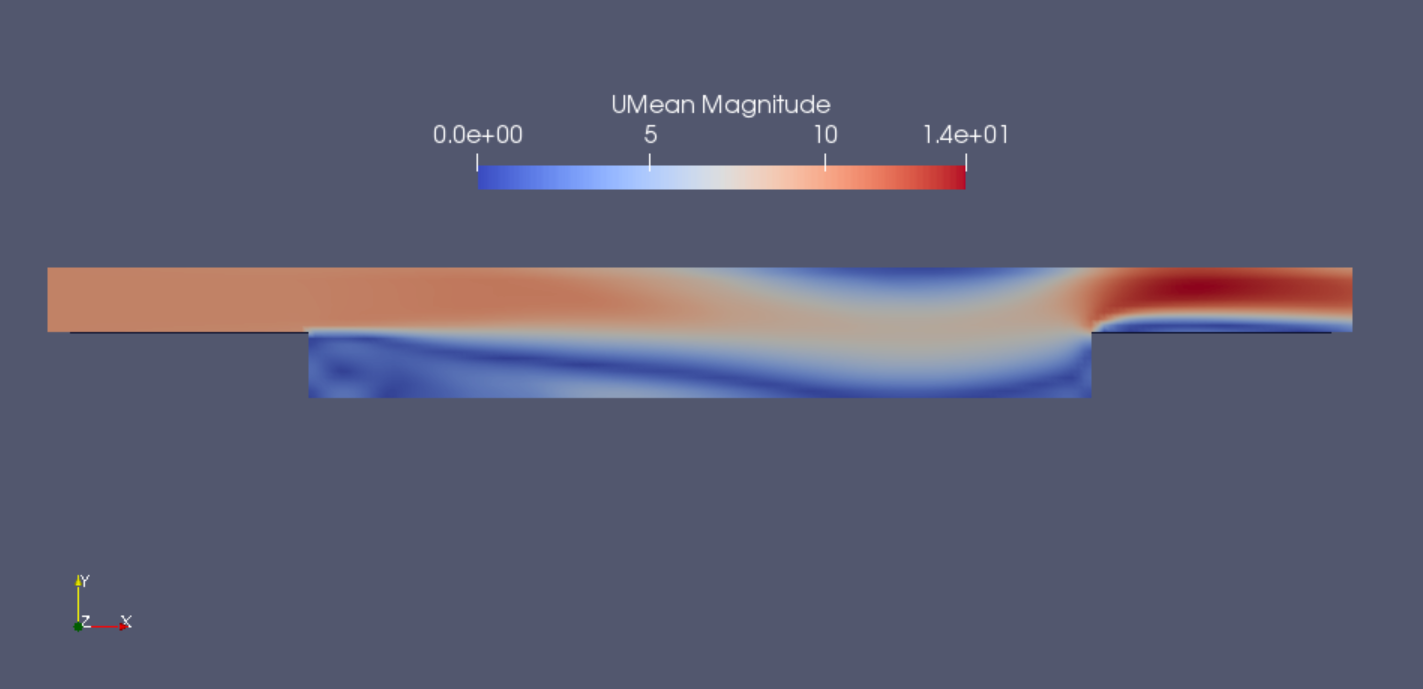
\includegraphics[width=0.6\linewidth]{Figures/piso_U_mean}
        \caption{Mean velocity magnitude, piso solver}
        \label{fig:MeanUPiso}
    \end{figure}

    \begin{figure}[h!]
        \centering
        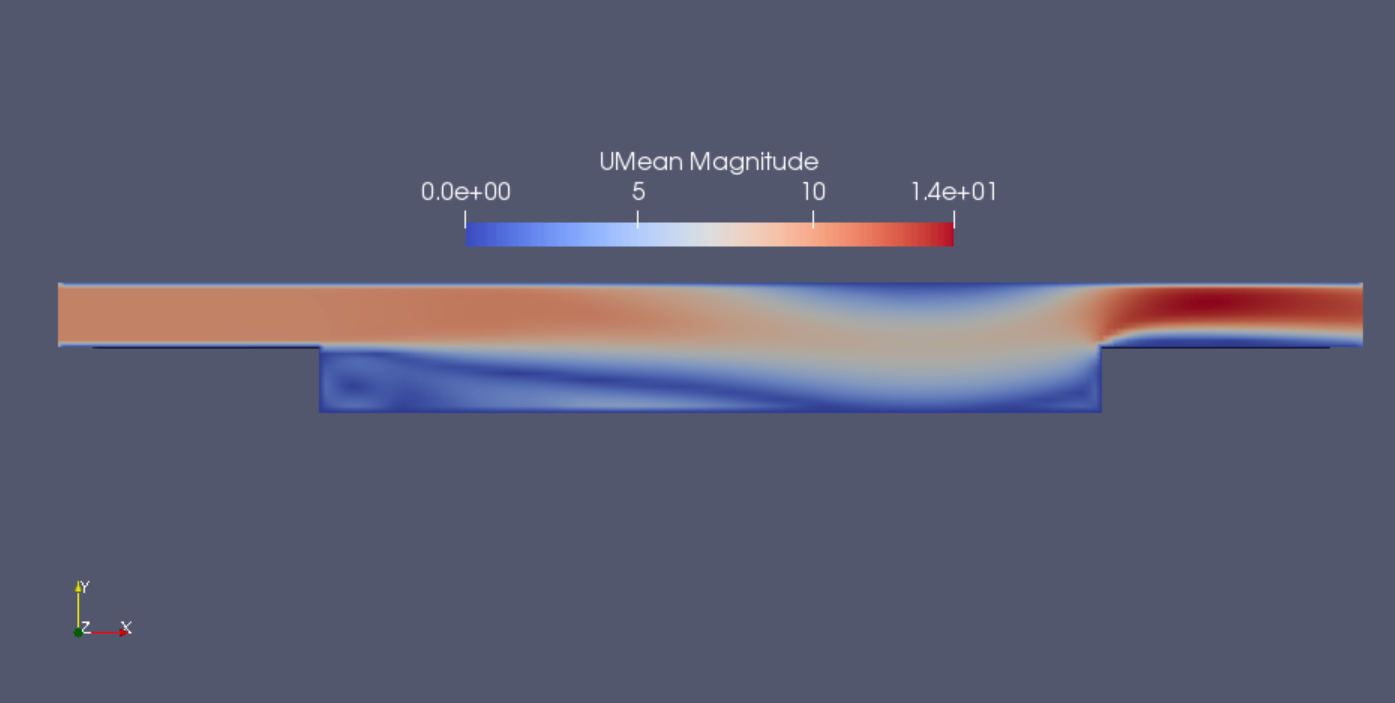
\includegraphics[width=0.6\linewidth]{Figures/piso_refined_U_mean}
        \caption{Mean velocity magnitude, refined mesh}
        \label{fig:MeanUPisoRef}
    \end{figure}

    \begin{figure}[h!]
        \centering
        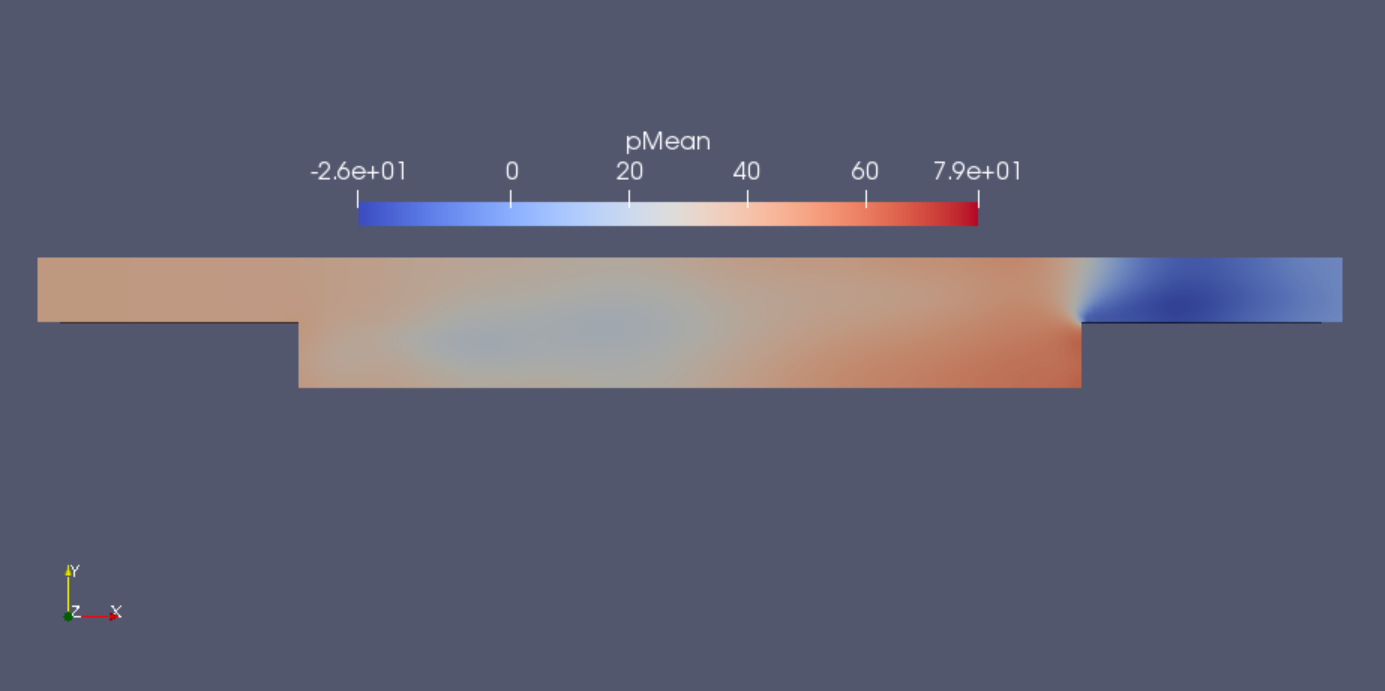
\includegraphics[width=0.6\linewidth]{Figures/piso_P_mean}
        \caption{Mean Pressure}
        \label{fig:MeanPPiso}
    \end{figure}

    \begin{figure}[h!]
        \centering
        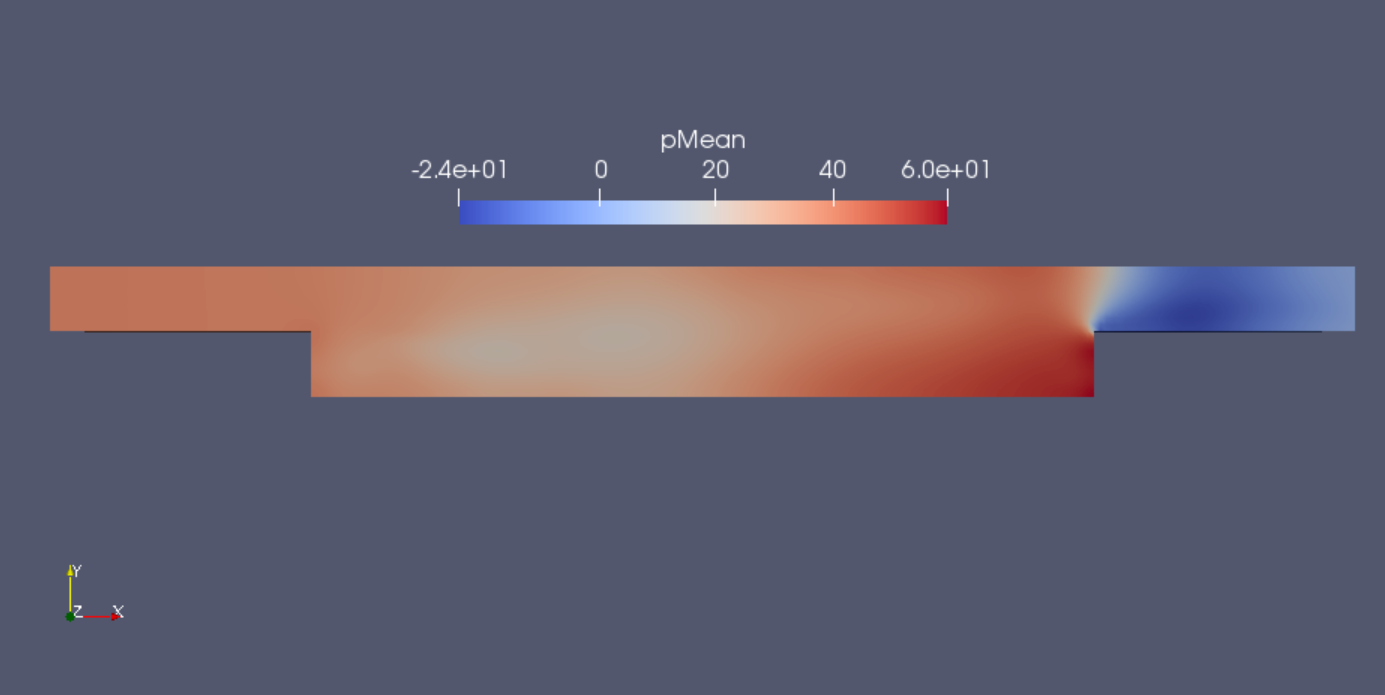
\includegraphics[width=0.6\linewidth]{Figures/piso_refined_P_mean}
        \caption{Mean Pressure, refined mesh}
        \label{fig:MeanPPisoRef}
    \end{figure}

    From figure \ref{fig:MeanUPiso} and \ref{fig:MeanUPisoRef} we can see that even with a doubling of control volume cells, that the mean velocity profile seems quite stable and mesh independent. similarly  in figures \ref{fig:MeanPPiso} and figure \ref{fig:MeanPPisoRef} we see that the mean pressure of the flow seems to also be mesh independent. 
    %----------------------------------------------------------------------------------------
    %  PROBLEM 2 - part 3
    %----------------------------------------------------------------------------------------
    
    \clearpage
    \subsection*{part 3}

    Having found a solution for the flow regime using LES and pisoFoam. We now attempt doing the same using two different RANS models and the simpleFoam solver. 


    The algorithm of simpleFoam can be found under incompressible solver, as the file simpleFoam.C. The base algorithm without turbulence modelling depends on the functions included from header files in this file, and in perticular the functions from the header files UEqn.H and pEqn.H. Below follows the simpleFoam file.
    
    
    \begin{lstlisting}[language=C++, captionpos=b, caption = source code for SimpleFoam]
        \*---------------------------------------------------------------------------*/

        #include "fvCFD.H"
        #include "singlePhaseTransportModel.H"
        #include "turbulentTransportModel.H"
        #include "simpleControl.H"
        #include "fvOptions.H"

        // * * * * * * * * * * * * * * * * * * * * * * * * * * * * * * * * * * * * * //

        int main(int argc, char *argv[])
        {
            #include "postProcess.H"

            #include "setRootCase.H"
            #include "createTime.H"
            #include "createMesh.H"
            #include "createControl.H"
            #include "createFields.H"
            #include "createFvOptions.H"
            #include "initContinuityErrs.H"

            turbulence->validate();

            // * * * * * * * * * * * * * * * * * * * * * * * * * * * * * * * * * * * //

            Info<< "\nStarting time loop\n" << endl;

            while (simple.loop())
            {
                Info<< "Time = " << runTime.timeName() << nl << endl;

                // --- Pressure-velocity SIMPLE corrector
                {
                    #include "UEqn.H"
                    #include "pEqn.H"
                }

                laminarTransport.correct();
                turbulence->correct();

                runTime.write();

                Info<< "ExecutionTime = " << runTime.elapsedCpuTime() << " s"
                    << "  ClockTime = " << runTime.elapsedClockTime() << " s"
                    << nl << endl;
            }

            Info<< "End\n" << endl;

            return 0;
        }


        // ************************************************************************* //
    \end{lstlisting}


    We can see in the simple loop structure that the velocity and pressure update and correction functions are included from their respectice header files. The Pressure correction equation can be found in the following code snippet.
    
    \begin{lstlisting}[language=C++]
        fvm::laplacian(rAtU(), p) == fvc::div(phiHbyA)
    \end{lstlisting}
    
    and its associated momentum correction equation:

    \begin{lstlisting}[language=C++]
        U = HbyA - rAtU()*fvc::grad(p);
    \end{lstlisting}

    and similarly the function for the velocity guess equation is found in the UEqn.h header file 
    
    \begin{lstlisting}[language=C++]
        tmp<fvVectorMatrix> tUEqn
        (
            fvm::div(phi, U)
          + MRF.DDt(U)
          + turbulence->divDevReff(U)
         ==
            fvOptions(U)
        );
    \end{lstlisting}

    And velocity is updated in the simpleFoam.C loop, using the equation

    \begin{lstlisting}[language=C++]
        solve(UEqn == -fvc::grad(p));
    \end{lstlisting}

    The boundary conditions used for the simpleFoam solver, can be found on the github link in the appendix. 
    In the following figures we see the results for mean velocity and mean kinetic energy for both a corse and a finer mesh.

    \begin{figure}[h]
        \centering
        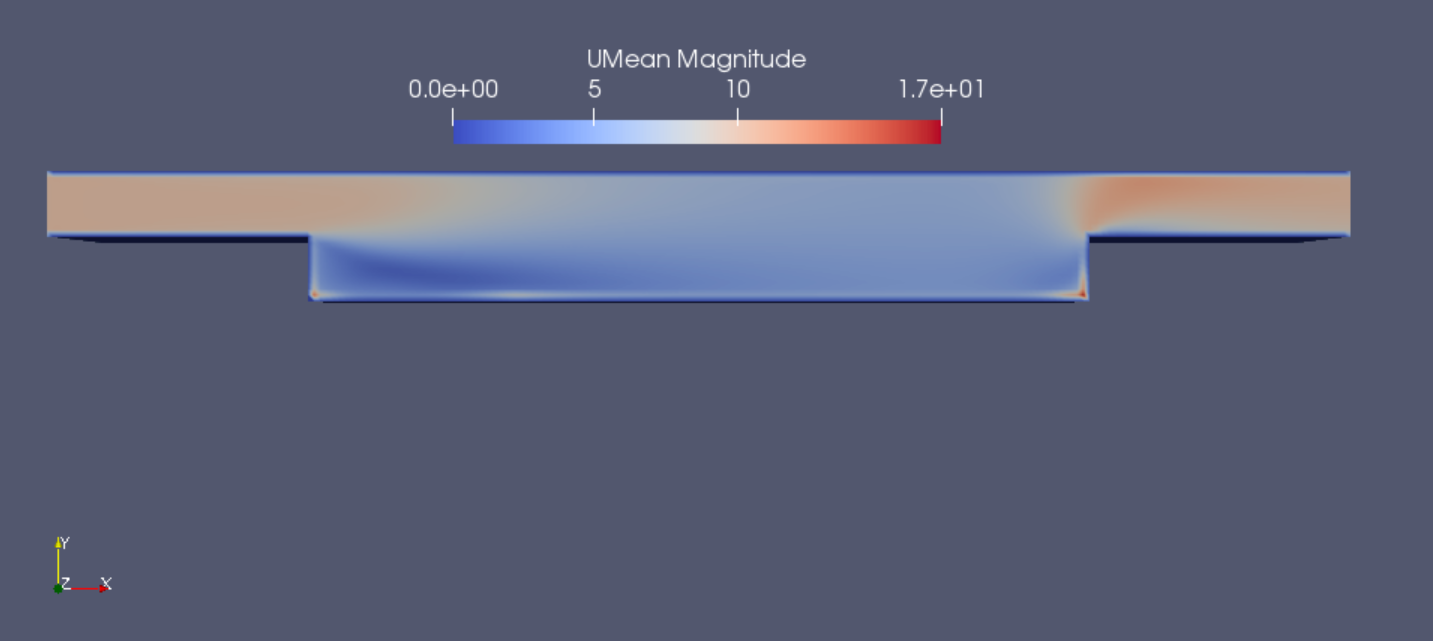
\includegraphics[width=0.6\linewidth]{Figures/simple_U_mean}
        \caption{Mean velocity magnitude $K - \epsilon$ turbulence}
        \label{fig:MeanUSimple}
    \end{figure}

    \begin{figure}[H]
        \centering
        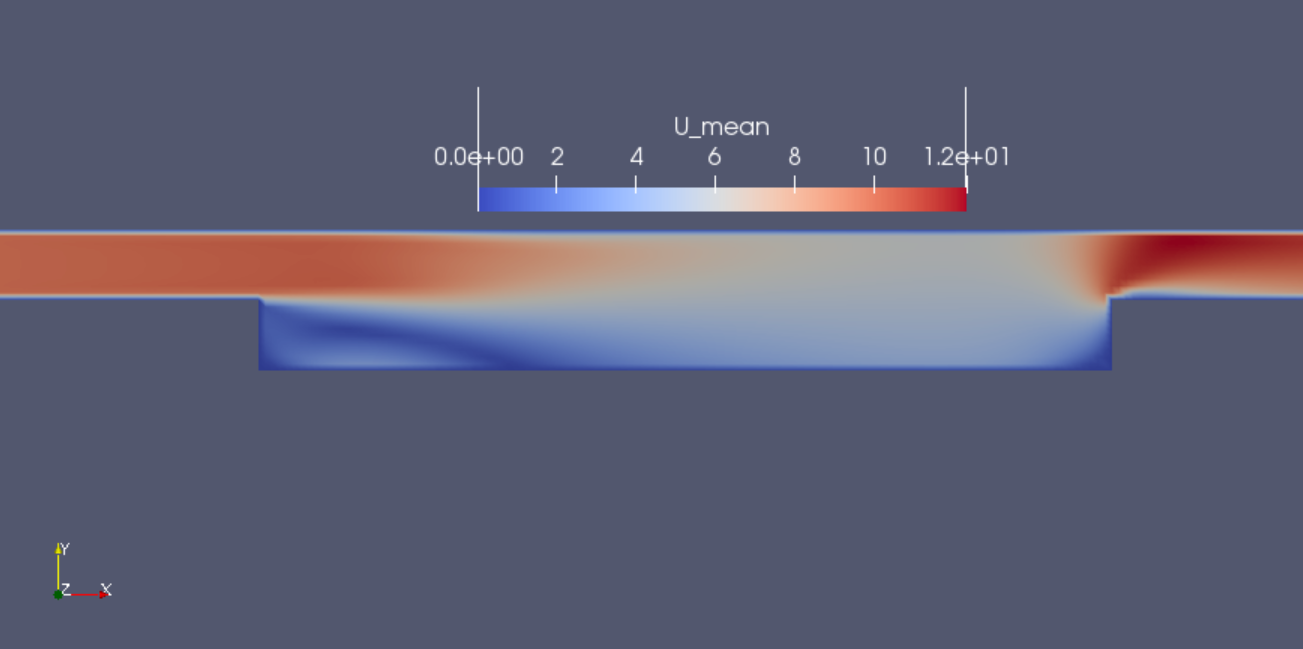
\includegraphics[width=0.6\linewidth]{Figures/simple_refined_U_mean}
        \caption{Mean velocity magnitude, refined mesh}
        \label{fig:MeanUSimpleRef}
    \end{figure}

    \begin{figure}[h]
        \centering
        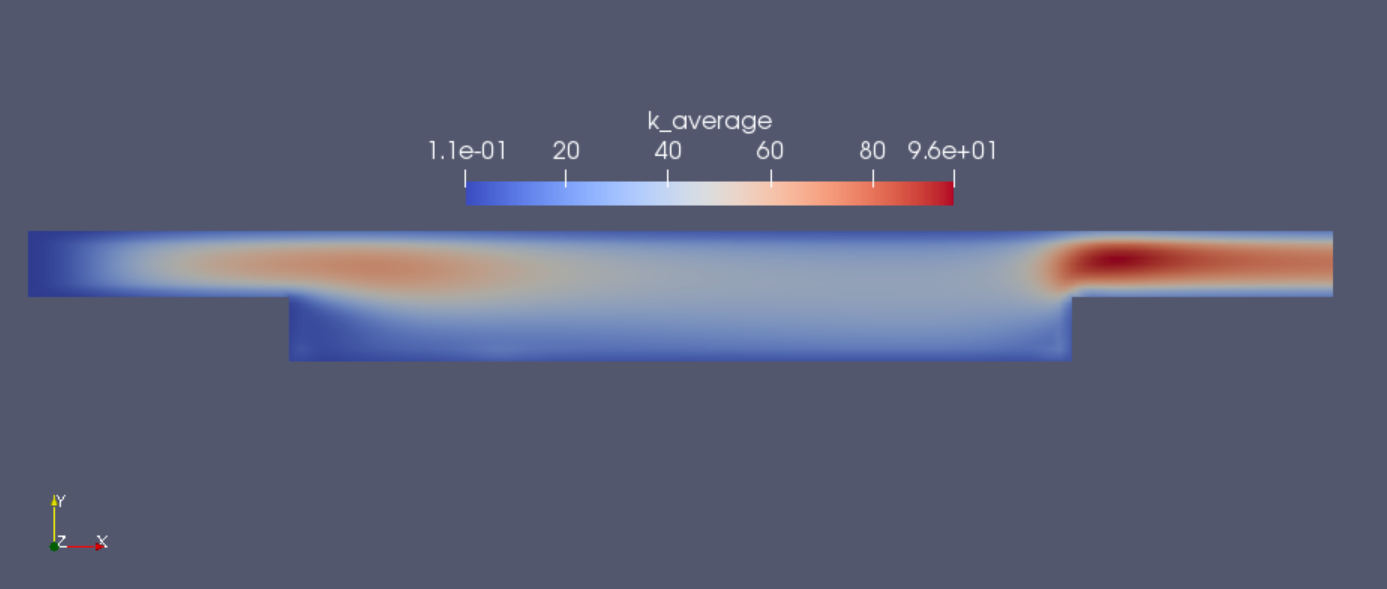
\includegraphics[width=0.6\linewidth]{Figures/simple_K_mean}
        \caption{Mean kinetic energy $K - \epsilon$ turbulence}
        \label{fig:MeanKSimple}
    \end{figure}

    \begin{figure}[H]
        \centering
        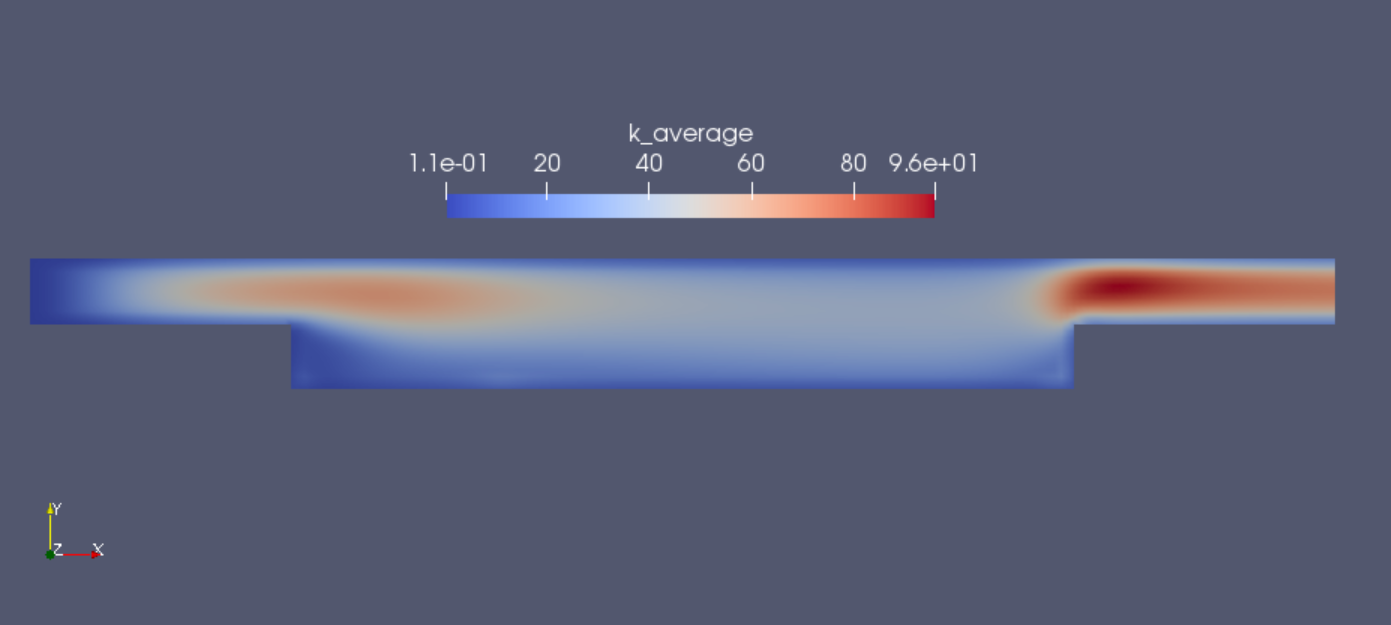
\includegraphics[width=0.6\linewidth]{Figures/simple_refined_K_mean}
        \caption{Mean kinetic energy, refined mesh}
        \label{fig:MeanKSimpleRef}
    \end{figure}

    \begin{figure}[H]
        \centering
        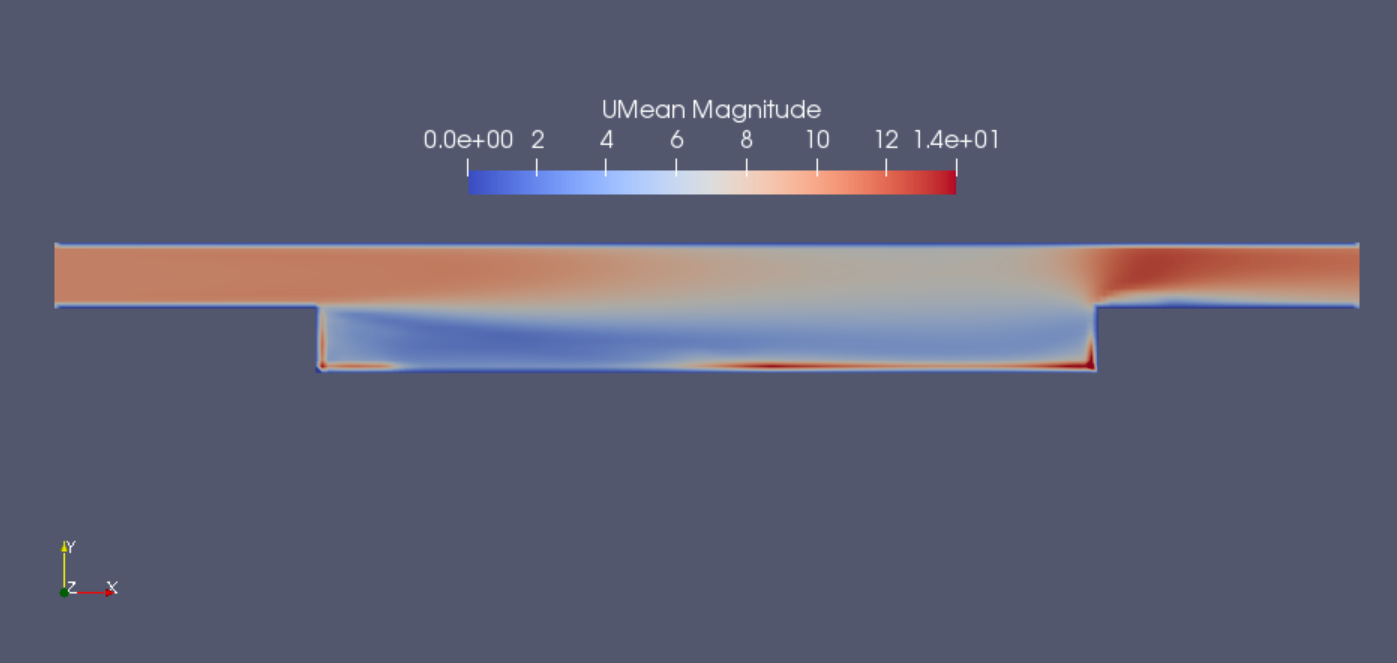
\includegraphics[width=0.6\linewidth]{Figures/simple_KOmega_U_mean}
        \caption{Mean velocity magnitude, $K - \omega$ turbulence}
        \label{fig:MeanUKOmega}
    \end{figure}

    \begin{figure}[H]
        \centering
        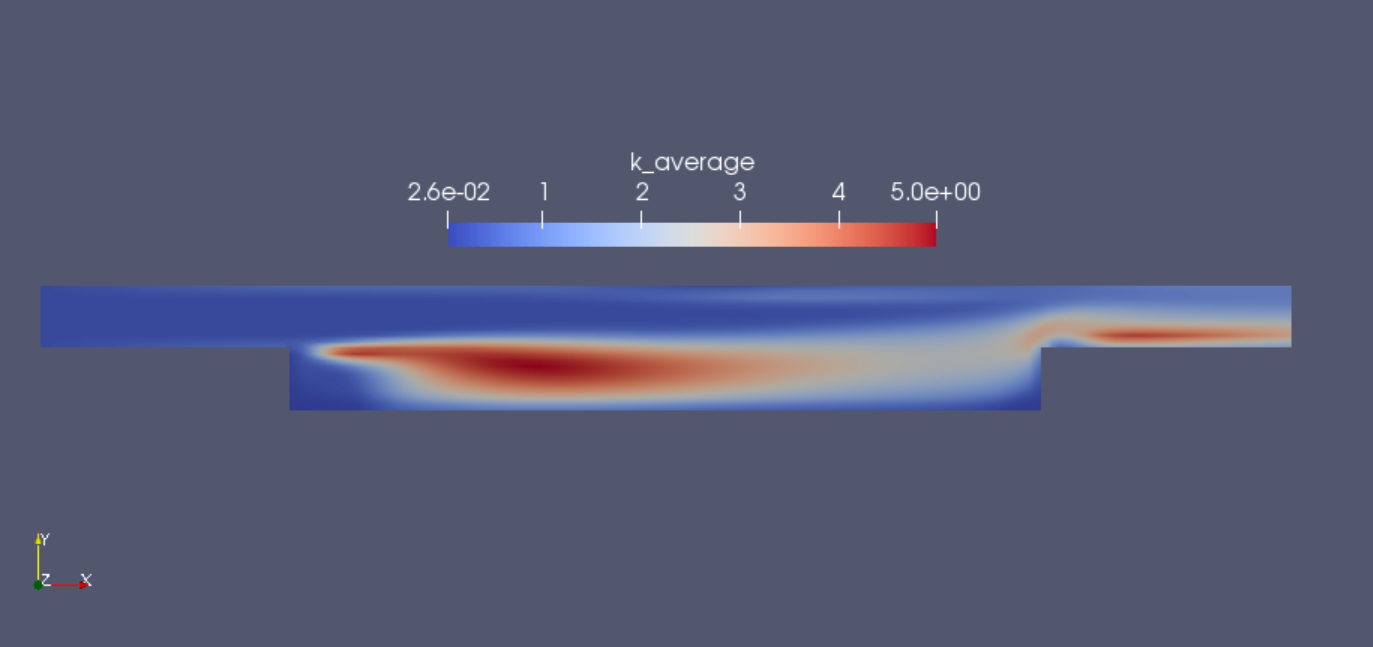
\includegraphics[width=0.6\linewidth]{Figures/simple_KOmega_K_mean}
        \caption{Mean kinetic energy, $K - \omega$ turbulence}
        \label{fig:MeanKKomega}
    \end{figure}
    %----------------------------------------------------------------------------------------
    %  PROBLEM 2 - part 4
    %----------------------------------------------------------------------------------------
    \clearpage
    \subsection*{part 4}
    To accurately compute turbulent flow using the LES model, a small $\Delta t$ is needed, pimpleFoam is however less stable for very small $\Delta t$, and is therefore more suitable for RANS modelling.
    
    %----------------------------------------------------------------------------------------
    %  PROBLEM 2 - part 5
    %----------------------------------------------------------------------------------------  
    \subsection*{part 5}
    We can get a visual sense of the accuracy of the computed solutions for $\overrightarrow{u}$ by comparing the respective locations for the recirculation bubble for both LES and RANS. We can visualize the recirculation bubble by applying contour lines on the velocity magnitude in paraview. Below follows the contour plot for velocity magnitude for LES/pisoFoam.

    \begin{figure}[h]
        \centering
        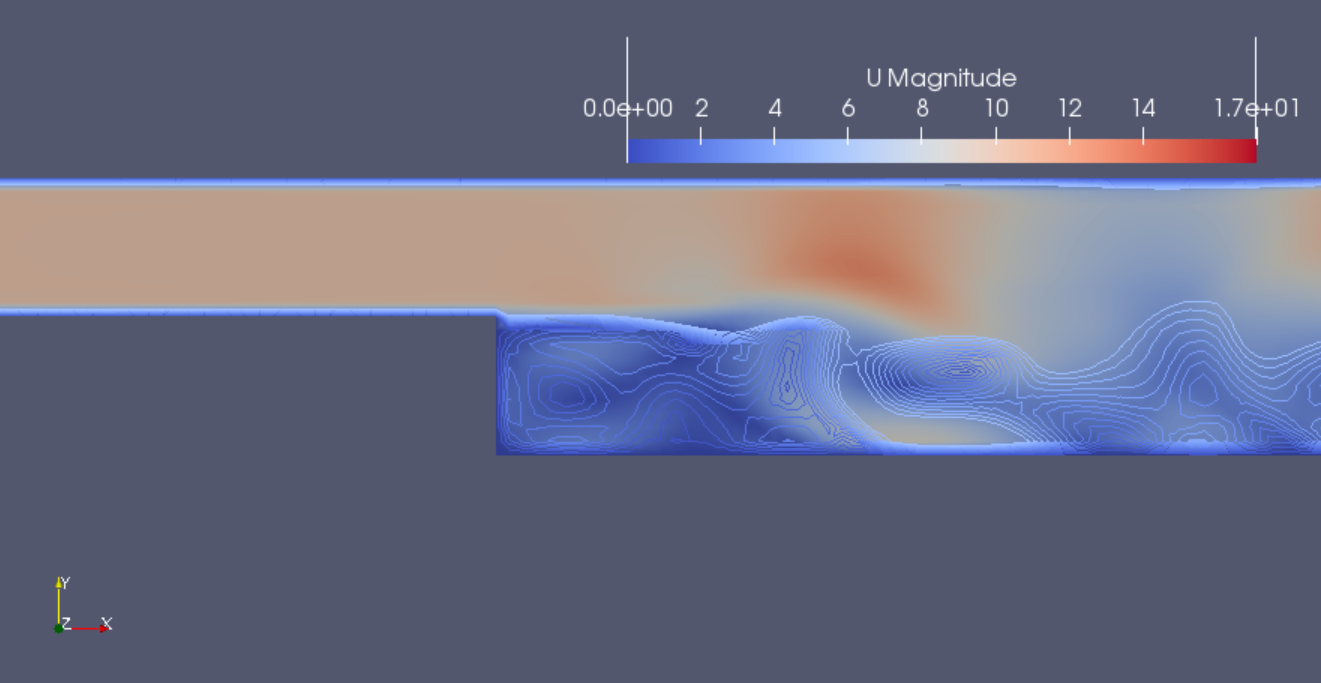
\includegraphics[width=0.6\linewidth]{Figures/isolines_U_mag_pisoFoam_refined}
        \caption{Isolines of velocity, pisoFoam}
        \label{fig:IsoPiso}
    \end{figure}
    
    And similarly for the $K-\epsilon$ RANS, SimpleFoam solution:

    \begin{figure}[h!]
        \centering
        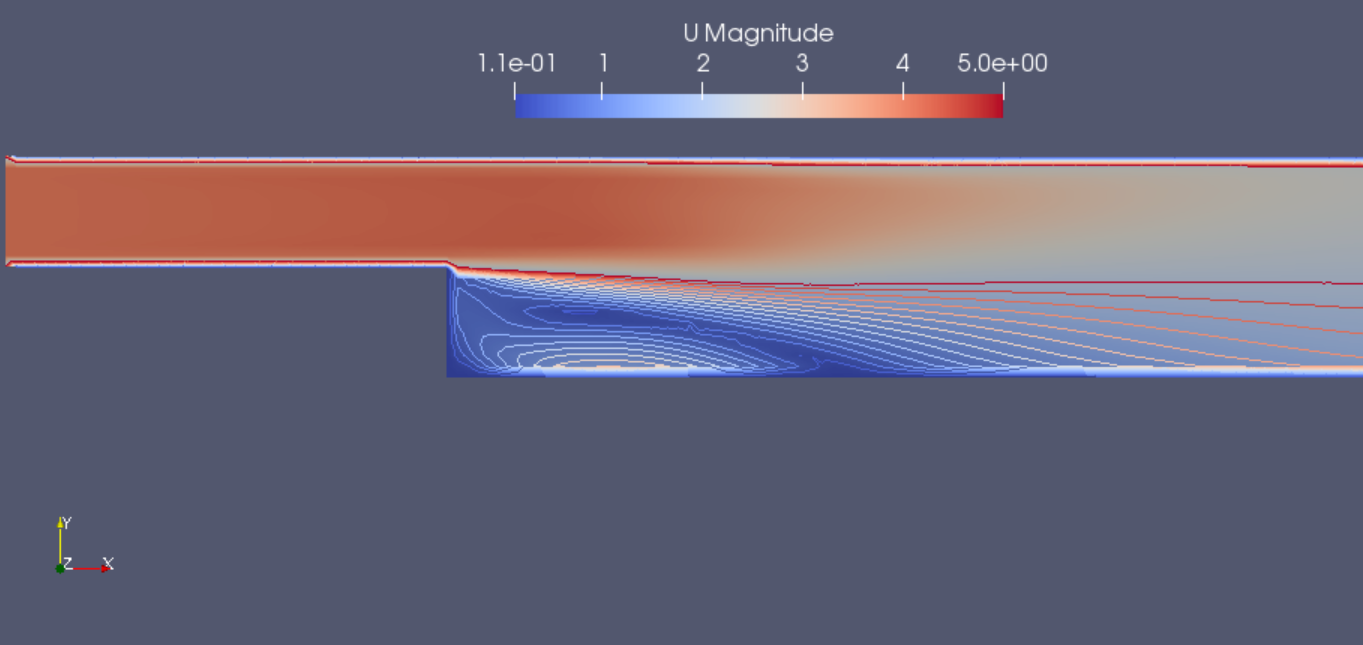
\includegraphics[width=0.6\linewidth]{Figures/isolines_U_mag_simpleFoam}
        \caption{Isolines of velocity, simpleFoam}
        \label{fig:IsoSimple}
    \end{figure}

    We can see in figure \ref{fig:IsoPiso} that the RANS solutions is able to accurately model the recirculation bubble as circular. The bubble also appears closer to the left wall, and higher up from the lower wall. In figure \ref{fig:IsoSimple} we see the bubble has become more smeared out in the direction of flow, and appears closer to the lower wall. This might be because of a difference in how convection is modelled in the respective turbulence models, and also due dissapation of turbulent energy in the case of LES.
    %----------------------------------------------------------------------------------------
    %  PROBLEM 2 - part 6
    %----------------------------------------------------------------------------------------

    \subsection*{part 6}
    The method of Large Eddy Simulations is a method of modelling turbulence. By using a corser mesh we can effectively filter out the smaller pertubations in the flow, yet capture the larger turbulent eddies in the flow; hence the name. Turbulence is inherently a three dimensional phenomena, since the LES model computes $\overrightarrow{u}(\overrightarrow{x}, t)$, a 3D geometry is required to accurately model the turbulent flow.
    %----------------------------------------------------------------------------------------
    %  Appendix
    %----------------------------------------------------------------------------------------
    \clearpage
    \section{Appendix}
    \subsection{TVD Code}
    \lstset{frame=tb,
    language=Python,
    breaklines=true,
    showstringspaces=false,
    columns=flexible,
    numbers=none,
    tabsize=4
    }
    \begin{center}
        
        \begin{lstlisting}[language=Python, captionpos = b, caption=Source code for excercise 1]
        '''
        example 5.1
        Upwind/Hybrid/Power-law/QUICK
        chapter: 5.6/5.7/5.8/5.9
        include L^2 feil
        '''
        from numpy import *
        from pylab import *

        def central_diff(N):
            faces = linspace(0, 1., N+1)
            nodes = 0.5*(faces[1:] + faces[:-1])
            delta = faces[1]-faces[0]

            # constants
            L = 1.0
            phi_a = 1.0
            phi_b = 0.0
            F = 0.1 # rho*u
            D = 0.1 / (1.0/N) # gamma/dx

            # Set up linear system of equations
            A = zeros((N, N))
            b = zeros(N)
            

            r = zeros(N)
            r = zeros(N)
            r[0] = 0
            r[-1] = 0

            lim = zeros(N) #limiter function
            lim[0]= 0
            lim[-1] = 0

            phi = linspace(1.,0.,N) 
            phi[0] = phi_a
            phi[-1] = phi_b

            for i in range(1,N-1):
                r[i] = (phi[i] - phi[i-1]) / (phi[i+1] - phi[i]) #Van Leer limiter
                lim[i] = (r[i] + abs(r[i])) / (1 + abs(r[i]))
            
            # ap*T_P - aw*T_W - ae*T_E = 0
            for i in range(1, N-1):
                aw = D + F/2
                ae = D - F/2
                sp = 0
                su = -F*(0.5*lim[i]*(phi[i+1] - phi[i]))
                ap = aw + ae - sp
                A[i, i-1] = -aw
                A[i, i]   = ap
                A[i, i+1] = -ae
                b[i] = su

            # Node 1
            ae = D - F/2
            aw = 0
            sp = -(2*D + F)
            su = (2*D + F) * phi_a
            ap = aw + ae - sp
            A[0, 0] = ap
            A[0, 1] = -ae
            b[0] = su

            # Node N add TVD
            aw = D + F/2
            ae = 0
            sp = -(2*D - F)
            su = (2*D - F) * phi_b
            ap = aw + ae - sp
            A[-1, -1] = ap
            A[-1, -2] = -aw
            b[-1] = su

            return nodes,A,b
                


        def Upwind(N):
            faces = linspace(0, 1., N+1)
            nodes = 0.5*(faces[1:] + faces[:-1])
            delta = faces[1]-faces[0]

            # constants
            L = 1.0
            phi_a = 1.0
            phi_b = 0.0
            F = 0.1 # rho*u
            D = 0.1 / (1.0/N) # gamma/dx

            # Set up linear system of equations
            A = zeros((N, N))
            b = zeros(N)

            # ap*T_P - aw*T_W - ae*T_E = 0
            for i in range(1, N-1):
                aw = D + F
                ae = D
                sp = 0
                su = 0
                ap = aw + ae - sp
                A[i, i-1] = -aw
                A[i, i]   = ap
                A[i, i+1] = -ae
                b[i] = su

            # Node 1, TVD corrected
            ae = D
            aw = 0
            sp = -(2*D + F)
            su = (2*D + F) * phi_a
            ap = aw + ae - sp
            A[0, 0] = ap
            A[0, 1] = -ae
            b[0] = su

            # Node N
            aw = D + F
            ae = 0
            sp = -2*D
            su = 2*D*phi_b
            ap = aw + ae - sp
            A[-1, -1] = ap
            A[-1, -2] = -aw
            b[-1] = su
            return nodes,A,b


        def QUICK(N):
            faces = linspace(0, 1., N+1)
            nodes = 0.5*(faces[1:] + faces[:-1])
            delta = faces[1]-faces[0]

            # constants
            L = 1.0
            phi_a = 1.0
            phi_b = 0.0
            F = 0.2 # rho*u
            D = 0.1 / (1.0/N) # gamma/dx

            # Set up linear system of equations
            A = zeros((N, N))
            b = zeros(N)

            for i in range(2, N-1):
                aw = D + (6/8)*F + (1/8)*F
                aww = -(1/8)*F
                ae = D - (3/8)*F
                aee = 0
                ap = aw + ae + aww + aee
                sp = 0
                su = 0
                A[i, i-1] = -aw
                A[i, i-2] = -aww
                A[i, i]   = ap
                A[i, i+1] = -ae
                b[i] = su

            # Node 1
            ae = D + (1/3)*D - (3/8)*F
            aw = 0
            aww = 0
            sp = -((8/3)*D + (2/8)*F + F)
            su = ((8/3)*D + (2/8)*F + F) * phi_a
            ap = aww + aw + ae - sp
            A[0, 0] = ap
            A[0, 1] = -ae
            b[0] = su

            # Node 2
            ae = D - (3/8)*F
            aw = D + (7/8)*F + (1/8)*F
            aww = 0
            sp = 0.25*F
            su = -0.25*F*phi_a
            ap = aww + aw + ae - sp
            A[1, 1] = ap
            A[1, 0] = -aw
            A[1, 2] = -ae
            b[1] = su
            

            # Node N
            aw = D + (1/3)*D + (6/8)*F
            aww = -(1/8)*F
            ae = 0
            sp = -((8/3)*D - F)
            su = ((8/3)*D - F)*phi_b
            ap = aww + aw + ae - sp
            A[-1, -1] = ap
            A[-1, -2] = -aw
            A[-1, -3] = -aww
            b[-1] = su
            return nodes,A,b

        def analytical(x_):
            F=0.2
            return (-1 * (exp(F * (x_/0.1)) - 1) / (exp(F * (1.0/0.1)) - 1)) + 1

        def L2_norm(num, anal, N):
            #return linalg.norm(num - anal)
            return linalg.norm(num-anal,2) #sqrt(1/N * sum((num - anal)**2))

        if __name__ == '__main__':
            err = []
            N = list(range(5,21))

            for i in N:
                nodes,A,b = central_diff(i)
                T = solve(A, b)
                exact = analytical(nodes)
                err.append(L2_norm(T,exact, i))
            print(T)
            figure(1)
            subplot(211)
            plot(nodes, T, 'b')
            plot(nodes, exact, 'r')
            xlabel('X')
            ylabel('Phi')
            title('Phi distribution')

            subplot(212)
            loglog(1 / asarray(N), err)
            loglog(1 / asarray(N), err, 1 / asarray(N), err[0]*(1 / asarray(N) * N[0]))
            xlabel('h')
            ylabel('L2 Error')
            title('Error vs. h')
            tight_layout()
            show()
        \end{lstlisting}
    
    \end{center}

    \end{document}